\documentclass[../../main.tex]{subfiles}
 
\begin{document}

\begin{table}
\centering
\begin{tabular}{| c | c | c | c |}
\hline \hline
This course... & $N$ & Mean & Standard-devliation \\ \hline
had clear goals and objectives. & 21 & 3.76 & 1.04 \\ \hline
was academically challenging. & 21 & 4.57 & 0.75 \\ \hline
offered useful learning tools. & 21 & 4.29 & 1.01 \\ \hline
had clearly defined grading criteria. & 21 & 3.52 & 1.33 \\ \hline
improved my understanding of the material. & 21 & 3.48 & 1.36 \\ \hline
increased my interest in the subject. & 21 & 3.29 & 1.68 \\ \hline
I would recommend this course to others. & 21 & 3.19 & 1.57 \\ \hline
\hline
\end{tabular}
\caption{\label{tab:courses:intro_eval_1} Summary of questions 10-16 on the student evaluation form, for PHYS135A taught in Fall 2017.}
\end{table}

\begin{table}
\centering
\begin{tabular}{| c | c | c | c |}
\hline \hline
The professor... & $N$ & Mean & Standard-devliation \\ \hline
used class time effectively and demonstrated preparation for class. & 21 & 4.24 & 1.04 \\ \hline
had a teaching style and enthusiasm that strengthened my interest. & 21 & 3.52 & 1.33 \\ \hline
was able to explain complicated ideas. & 21 & 3.48 & 1.40 \\ \hline
challenged students to think critically and/or imaginatively. & 21 & 4.24 & 1.09 \\ \hline
provided clear and timely feedback. & 21 & 4.48 & 1.03 \\ \hline
encouraged meaningful class discussions. & 21 & 4.10 & 0.89 \\ \hline
receptive to differing views. & 21 & 3.95 & 1.20 \\ \hline
was available for help outside of class. & 21 & 4.67 & 0.58 \\ \hline
Overall, I would recommend this professor to others. & 21 & 3.24 & 1.55 \\ \hline
\hline
\end{tabular}
\caption{\label{tab:courses:intro_eval_2} Summary of questions 17-25 on the student evaluation form, for PHYS135A taught in Fall 2017.}
\end{table}

\begin{figure}
\centering
\includegraphics[width=0.33\textwidth,angle=270]{aggregate_data_fall_2017_intro.eps}
\includegraphics[width=0.33\textwidth,angle=270]{aggregate_data_spring_2018_intro.eps}
\caption{\label{fig:ag_data} (Left) Aggregate standard deviations versus mean scores for questions 10-25 for introductory courses taught in Fall 2017.  (Right) Same, for introductory courses taught in Spring 2018.}
\end{figure}

\end{document}

